\documentclass[11pt,a4paper]{article}
\usepackage[a4paper,margin=24mm]{geometry}
\usepackage[T1]{fontenc}
\usepackage[utf8]{inputenc}
\usepackage{lmodern}
\usepackage{amsmath,amssymb,amsthm}
\usepackage{graphicx}
\usepackage{booktabs,array,tabularx,multirow}
\usepackage[font=small,labelfont=bf]{caption}
\usepackage{enumitem}
\usepackage{microtype}
\usepackage{xcolor}
\definecolor{linkblue}{rgb}{0,0.15,0.5}
\usepackage[colorlinks=true,linkcolor=linkblue,citecolor=linkblue,urlcolor=linkblue]{hyperref}
\usepackage{url}
\graphicspath{{./}{figs/}{paper02_probabilistic_sufficiency_v16_src/figs/}}
\theoremstyle{plain}
\newtheorem{theorem}{Theorem}[section]
\newtheorem{proposition}[theorem]{Proposition}
\newtheorem{lemma}[theorem]{Lemma}
\newtheorem{corollary}[theorem]{Corollary}
\theoremstyle{definition}
\newtheorem{definition}[theorem]{Definition}
\newtheorem{example}[theorem]{Example}
\theoremstyle{remark}
\newtheorem{remark}[theorem]{Remark}
\newcommand{\R}{\mathbb{R}}
\newcommand{\Qr}{\mathbb{Q}}
\newcommand{\N}{\mathbb{N}}
\newcommand{\E}{\mathbb{E}}
\newcommand{\Prob}{\mathbb{P}}
\newcommand{\calV}{\mathcal{V}}
\newcommand{\calS}{\mathcal{S}}
\newcommand{\calW}{\mathcal{W}}
\newcommand{\calD}{\mathcal{D}}
\newcommand{\Wfb}{\calW^{\mathrm{fb}}}
\newcommand{\Wbl}{\calW^{\mathrm{bl}}}
\newcommand{\supp}{\operatorname{supp}}
\newcommand{\Post}{\operatorname{Post}}
\newcommand{\hold}{\mathrm{hold}}
\newcommand{\ol}{\mathrm{ol}}
\newcommand{\seq}{\mathrm{seq}}
\newcommand{\obs}{\mathrm{obs}}
\newcommand{\Tobs}{T_{\mathrm{obs}}}
\newcommand{\Tl}{T_{\mathrm{learn}}}
\newcommand{\ind}[1]{\mathbf{1}[#1]}
\newcommand{\tfr}[2]{\tfrac{#1}{#2}}
\setlength{\parskip}{2pt}
\emergencystretch=2em
\allowdisplaybreaks

\begin{document}

\title{\textbf{Probabilistic sufficiency under partial observation:\\ belief-state safety values, survivable-set antichains,\\ and the exact price of late information}}
\author{Amin Abaee\\[0.3em]
{\small Independent Researcher}\\[0.2em]
{\small ORCID: \href{https://orcid.org/0000-0002-0019-1842}{0000-0002-0019-1842}\quad
\href{mailto:amin_abaee@ut.ac.ir}{amin\_abaee@ut.ac.ir}}}
\date{October 15, 2026}
\maketitle

\begin{abstract}
\noindent
Set-valued viability theory under incomplete observation delivers binary verdicts: an information state is viable or it is obstructed. This paper develops the quantitative counterpart, the belief-state safety value $V_k(b)$---the maximal probability, over a declared policy class, of keeping the state in the safe set for $k$ steps when the controller holds a distribution $b$ over states---and carries it entirely in exact rational arithmetic. Three structural results connect the two theories. First, on finite models with deterministic kernels and deterministic observation maps the posterior support follows the set-valued post-state exactly, so $V_k(b)=1$ holds precisely when the support lies in the feedback viable-set recursion, and otherwise the deficit obeys $1-V_k(b)\ge\min_{x\in\supp b}b(x)$; the condition is necessary as well as sufficient, in contrast to the sufficient-only output-feedback criteria of the viability literature. Second, the $\alpha$-vectors of the value are exactly the indicators of the maximal jointly survivable subsets of the support---an antichain, Sperner-bounded, the bound being attained---and the value of observation over blind control is at most $1-\max_x b(x)$, a bound attained for every support size. Third, on a delayed hidden-regime class the hold-class, open-loop and fully observed values are obtained in closed form for all initial states, window lengths, horizons and prior weights; the class lattice orders them, and the two gaps---the value of flexibility and the value of observation---are each $\min(w,1-w)$ on disjoint, explicitly located cells. The classical timing obstruction is thereby shown to be a statement about the declared hold class, exactly on the cells where open-loop time variation restores safety. Beyond the deterministic layer, observation becomes a design variable: a pinned probe of a hidden drift parameter at deadline $T$ moves the viability threshold linearly, $z_0\ge\tfrac{21}{10}+\tfrac{T}{10}$, between a flat free-probe benchmark and a probe-free one, and a general hold--probe--learn schedule has an exact threshold that reduces to an additive law under aligned worst losses. Under noisy sensing the deficit is the prior mass weighted by fatal-reading probabilities, a two-state sensor attains deficit $\tfrac1{20}$ against a minimal mass of $\tfrac12$, a single noisy probe yields exactly three value levels, and $n$ repeated readings bring the wrong-majority probability below $(4\varepsilon(1-\varepsilon))^{n/2}$ at a cost of one unit of floor margin per reading. A contamination operator interpolates exactly between the expected and worst-case readings at one stage, but not across stages, and admits a closed form on the delayed class. Every statement is regenerated from the definitions by a deterministic exact-arithmetic script; the support identity, the stabilization count and the rationality of the $\alpha$-vectors are additionally machine-checked in Lean~4.
\end{abstract}

\medskip
\noindent\textbf{Keywords:} partially observable Markov decision processes; stochastic viability; safety probability; belief states; $\alpha$-vectors; value of information; learning deadlines; exact rational verification

\medskip
\noindent\textbf{MSC 2020:} 93E20, 90C40, 93B07, 49N30, 60J20

\section{Introduction}\label{sec:intro}

A controller that must keep a system inside a safe set, but cannot see the state, faces two questions. The first is qualitative: does the information available suffice, in principle, to guarantee safety? The second is quantitative: when it does not, how much safety survives? Viability theory answers the first question with set-valued objects---viability kernels, regulation maps and, under incomplete observation, obstruction certificates that prove an information state nonviable \cite{Aubin1991,Veliov1993,Doyen2000,Abaee2026calc}. Stochastic viability \cite{DeLaraDoyen2008,DoyenDeLara2010} and probabilistic reachability \cite{Abate2008} answer the second question under full observation, by a dynamic programme for the maximal probability of remaining in the constraint set. The partially observed, quantitative case sits between the two: the information state is a probability distribution over states, a belief, and the natural object is the \emph{belief-state safety value}
\[
V^{\Pi}_{k}(b)\;=\;\sup_{\pi\in\Pi}\;\Prob_{\pi}\bigl(x_t\in\calV\ \text{for } t=0,\dots,k\;\big|\;b\bigr),
\]
the maximal probability, within a declared policy class $\Pi$, of surviving $k$ steps from the belief $b$. Its value-one level is a viability statement; everything below it is measured by the deficit $1-V^{\Pi}_k(b)$.

This paper develops $V^{\Pi}_k$ as an exact theory. The word \emph{exact} is meant literally: every value, witness, threshold and count reported here is a rational number computed from the definitions in integer and rational arithmetic, and the structural theorems explain why the computations produce the numbers they do. The development has a deterministic layer, in which the kernels and observation maps are deterministic and the value measures how much prior mass a policy can keep alive, and a stochastic layer, in which sensing is noisy and the value is a genuine probability.

\paragraph{Contributions.}
\begin{enumerate}[leftmargin=1.6em,itemsep=1pt]
\item \emph{Exact sufficiency} (Theorem~\ref{thm:support}). On finite models with deterministic kernels and deterministic observation maps the support of the Bayesian posterior equals the set-valued post-state of the obstruction calculus; hence $V_k(b)=1$ if and only if $\supp b$ belongs to the feedback viable-set recursion $\Wfb_k$, and otherwise $1-V_k(b)\ge\min_{x\in\supp b}b(x)$. The criterion is necessary as well as sufficient, where the nearest output-feedback criterion of the viability literature \cite{Veliov1993} is sufficient only, and it admits history-dependent policies, where the necessary-and-sufficient criterion of \cite{Doyen2000} is confined to memoryless Lipschitz loops. The feedback and blind recursions differ, and the \emph{value of observation} $V^{\seq}_k-V^{\ol}_k$ is at most $1-\max_x b(x)$ whenever every state is individually survivable, a bound attained for every support size (Proposition~\ref{prop:feedback}).
\item \emph{The survivable-set antichain} (Theorem~\ref{thm:antichain}). Under deterministic kernels the $\alpha$-vectors of the value are exactly the indicators of the maximal jointly survivable subsets of the support. These form an antichain, so their number is at most $\binom{n}{\lfloor n/2\rfloor}$ for a support of size $n$ (Sperner), the bound is attained, and the deficit is $\min_S b(S^{c})$ over the maximal sets. This explains the three-type witness census of the certified instances and gives the value a finite, enumerable structure; the value stabilizes in the horizon after at most $2^{n}$ strict decreases (Proposition~\ref{prop:freeze}).
\item \emph{Certificates as deficit bounds} (Proposition~\ref{prop:deficit}). The chance-constrained common-action certificate, the minimal-mass certificate and horizon monotonicity are lower bounds on the exact deficit, attained on natural instances at symmetric and asymmetric priors.
\item \emph{Closed forms and the class lattice on the delayed hidden-regime class} (Theorems~\ref{thm:closed} and~\ref{thm:lattice}). For a hidden regime revealed after a blind window of length $\Tobs$, the hold-class, open-loop and fully observed safety values are obtained in closed form for all initial states, horizons, window lengths and prior weights. The inclusion of classes orders the values, both gaps are realized exactly and on disjoint cells---the value of flexibility on $\{2\le z_0<1+\min(k,\Tobs)\}$ and the value of observation on $\{1\le z_0<2\}$, each equal to $\min(w,1-w)$---and the classical timing obstruction is identified as a statement about the declared hold class (Corollary~\ref{cor:timing}). The complete certified value table, its $36/156$ census and its $384$ witnesses ($348$ distinct) are corollaries (Corollary~\ref{cor:grid}).
\item \emph{The price of late information} (Section~\ref{sec:deadline}). When a hidden drift parameter can only be learned by probing, a probe pinned to the deadline $\Tl$ shifts the viability threshold linearly, $z_0\ge\tfrac{21}{10}+\tfrac{\Tl}{10}$, between a flat free-probe benchmark and a probe-free one (Proposition~\ref{prop:deadline}); a general hold--probe--learn schedule has an exact threshold which reduces to an additive worst-loss law when the worst hold loss and the worst probe excursion are attained by a common parameter value, and not otherwise (Theorem~\ref{thm:additive}).
\item \emph{The stochastic layer} (Section~\ref{sec:stochastic}). Under noisy sensing the one-step deficit is the prior mass weighted by fatal-reading probabilities; a two-state sensor instance attains deficit $\min\{\varepsilon,b(x_1),b(x_2)\}$, so the minimal-mass bound is a deterministic-limit statement and not a law of the noisy layer. A single noisy probe of the hidden drift yields exactly the three value levels $\{0,1-\varepsilon,1\}$; majority reading over $n$ probes drives the wrong-majority probability below $(4\varepsilon(1-\varepsilon))^{n/2}$ at the cost of one unit of floor margin per additional reading---an exact exploration--safety exchange.
\item \emph{Robust interpolation} (Section~\ref{sec:dr}). A contamination ambiguity set of radius $\rho$ interpolates exactly between the expected and the worst-case reading at one stage, the adversary spending its whole budget on the worst outcome; the interpolation does not extend affinely across stages (a two-stage instance gives $\tfrac1{16}$ against $\tfrac18$), and a prior-contamination model has a closed form on the delayed class.
\end{enumerate}

\paragraph{Relation to the companion papers.}
The set-valued theory this paper quantifies is the obstruction calculus of \cite{Abaee2026calc}; its finite certification and worked-systems audits are treated in \cite{Abaee2026cert,Abaee2026worked}, and its minimax dual certificates in \cite{Abaee2026minimax}. Nothing proved there is re-derived differently here; the interface is Proposition~\ref{prop:deficit}, which reads each certificate as a lower bound on the exact deficit, and Corollary~\ref{cor:timing}, which scopes the timing certificate to its policy class. The two running instances---the delayed hidden-regime instance and the two-floor instance---are shared with the calculus so that the quantitative values can be compared cell by cell with the set-valued verdicts.

\paragraph{Organisation.}
Section~\ref{sec:setting} fixes the model, the policy classes, the safety value and its exact $\alpha$-vector representation. Section~\ref{sec:support} proves the support identity, the antichain theorem and stabilization. Section~\ref{sec:deficit} reads the certificates as deficit bounds. Section~\ref{sec:delayed} treats the delayed hidden-regime class: closed forms, the class lattice, the scoping of the timing obstruction and the certified grid. Section~\ref{sec:deadline} prices late information, Section~\ref{sec:stochastic} opens the stochastic layer, and Section~\ref{sec:dr} develops the contamination interpolation. Section~\ref{sec:related} positions the results, Section~\ref{sec:verification} describes the exact verification and the machine-checked layer, and Section~\ref{sec:discussion} discusses limitations and consequences. The supplementary material (S1--S8) carries the complete certified table, the asymmetric audit, the derivations of the jump loci, the learning-deadline tables, the exact probe-count values, the proofs for the contamination operator, the verification record and a cross-paper symbol table.
\section{Setting: safety POMDPs, policy classes and the safety value}\label{sec:setting}

\subsection{The augmented model}

\begin{definition}[safety POMDP with absorbing unsafe state]\label{def:model}
A \emph{safety POMDP} consists of a finite safe set $\calV$, the augmented state space $X^{\bot}=\calV\cup\{\bot\}$ with an absorbing unsafe state $\bot$, a finite action set $A$, a finite observation set $Y^{\bot}=Y\cup\{y_{\bot}\}$, a transition kernel $T$ and an observation law $g$, all with rational data:
\begin{enumerate}[leftmargin=1.6em,itemsep=1pt]
\item for $x\in\calV$ and $a\in A$ the row $T(\cdot\mid x,a)$ is sub-stochastic on $\calV$, with \emph{exit probability} $p(x,a)=1-\sum_{x'\in\calV}T(x'\mid x,a)=T(\bot\mid x,a)$, and $T(\bot\mid\bot,a)=1$;
\item for $x,x'\in\calV$ the law $g(\cdot\mid x,a,x')$ is a probability distribution on $Y$, and the exit is announced: $g(y_{\bot}\mid\cdot,\cdot,\bot)=1$.
\end{enumerate}
A \emph{belief} is a probability distribution $b$ on $X^{\bot}$; only its restriction to $\calV$ matters for safety, and $b(\calV)=\sum_{x\in\calV}b(x)$ is the mass still alive. For $y\in Y$ the observation likelihood and the Bayes update are
\begin{gather*}
\Prob(y\mid b,a)=\sum_{x,x'\in\calV}b(x)\,T(x'\mid x,a)\,g(y\mid x,a,x'),\\
\tau(b,a,y)(x')=\frac{\sum_{x\in\calV}b(x)\,T(x'\mid x,a)\,g(y\mid x,a,x')}{\Prob(y\mid b,a)}\qquad(x'\in\calV),
\end{gather*}
defined when $\Prob(y\mid b,a)>0$, while $\tau(b,a,y_{\bot})=\delta_{\bot}$. Since every row sums to one and every transition emits exactly one observation, $\sum_{y\in Y^{\bot}}\Prob(y\mid b,a)=1$ at every belief: no sub-probability bookkeeping is needed, and exit from $\calV$ is absorption with no re-entry.
\end{definition}

The kernels are \emph{deterministic} if every row $T(\cdot\mid x,a)$ is a point mass, at some $F(x,a)\in\calV$ or at $\bot$; the observation maps are deterministic if $g(\cdot\mid x,a,x')$ is a point mass $\delta_{h(x,a,x')}$. Under both hypotheses the model is the set-valued model of the obstruction calculus \cite{Abaee2026calc} with a prior placed on the compatible states, and the \emph{post-state} of a set $B\subseteq\calV$ under $(a,y)$ is
\[
\Post(B,a,y)=\{F(x,a):x\in B,\ F(x,a)\in\calV,\ h(x,a,F(x,a))=y\}.
\]

\subsection{Policy classes and the safety value}

A history at stage $t$ is $h_t=(a_0,y_1,\dots,a_{t-1},y_t)$, and a (deterministic) policy maps the initial belief and the history to an action. Four classes recur.
\begin{itemize}[leftmargin=1.6em,itemsep=1pt]
\item $\Pi_{\seq}$: all history-dependent policies (the \emph{sequential} or feedback class).
\item $\Pi_{\ol}(\ell)$: policies whose actions on the window $t=0,\dots,\ell-1$ are fixed in advance, $a_t=u_t$, and unrestricted afterwards (\emph{open-loop} on the window). When the window is \emph{blind}---no observation other than the exit announcement arrives before stage $\ell$---the sequential and the open-loop classes coincide on the window, because the only history available is the observation-free one.
\item $\Pi_{\hold}(\ell)\subseteq\Pi_{\ol}(\ell)$: policies that hold one action $u_0=\dots=u_{\ell-1}=u$ on the window and are unrestricted afterwards (the \emph{hold} class, the institutional reading of a regulator who sets a rule and reviews it only at the end of the window).
\item $\Pi_{\obs}$: the sequential class under a finer information pattern in which the state is observed from the start; its value is the stochastic viability value under full observation \cite{DoyenDeLara2010} and serves as the upper benchmark.
\end{itemize}

\begin{definition}[safety value and its levels]\label{def:value}
For a class $\Pi$ and a horizon $k\ge0$ the \emph{safety value} is
\[
V^{\Pi}_{k}(b)=\max_{\pi\in\Pi}\ \Prob_{\pi}\bigl(x_t\in\calV\text{ for }t=0,\dots,k\;\big|\;b\bigr),
\]
the horizon counting the current state; the maximum exists because for finite horizon, action and observation sets finitely many deterministic policies compete, and randomization cannot increase a probability that is linear in the policy's stagewise mixtures. The \emph{deficit} is $\Delta^{\Pi}_k(b)=1-V^{\Pi}_k(b)$. The superscript is dropped for the sequential class. Two action sets at a belief must be distinguished: the \emph{attaining set} $\Gamma^{\mathrm s}_k(b)$ of actions achieving the maximum in the recursion below, which is nonempty at every belief and carries no viability content, and the \emph{value-one level} $S_k(b)$ of actions after which the continuation value is one, whose nonemptiness is equivalent to $V_k(b)=1$. Obstruction certificates correspond to $S_k(b)=\varnothing$.
\end{definition}

\begin{proposition}[belief-state recursion]\label{prop:recursion}
$V_0(b)=b(\calV)$ and, for $k\ge0$,
\begin{equation}\label{eq:recursion}
V_{k+1}(b)=\max_{a\in A}\ \sum_{y\in Y}\Prob(y\mid b,a)\,V_{k}\bigl(\tau(b,a,y)\bigr),
\end{equation}
the exit observation contributing zero. The same recursion with the stagewise admissible set $A_t(\Pi)$ in place of $A$ computes $V^{\Pi}_k$ for every class defined by stagewise action restrictions; for the window classes $\Pi_{\ol}(\ell)$ and $\Pi_{\hold}(\ell)$, whose constraint couples the stages of the window, the equivalent segment form of Proposition~\ref{prop:alpha} applies on the window and \eqref{eq:recursion} after it.
\end{proposition}

\begin{proof}
This is value iteration for the belief-state Markov decision process \cite{Astrom1965,SmallwoodSondik1973,BertsekasShreve1978} with the multiplicative survival objective: conditioning on the first action and observation, the probability of surviving $k+1$ stages is the probability of surviving the first transition and the observation-weighted probability of surviving $k$ further stages from the posterior, and $\bot$ is absorbing, so the exit branch contributes zero. The partially observed multiplicative recursion is the finite-state case of the sufficient-statistic construction of \cite{LesserOishi2014}. For a window class, enumerate the admissible window segments and apply \eqref{eq:recursion} to the continuation.
\end{proof}

\subsection{Exact $\alpha$-vector representation}

\begin{proposition}[rational $\alpha$-vectors]\label{prop:alpha}
Fix a class $\Pi$ with stagewise admissible sets. At every horizon $k$ the value is piecewise linear and convex in $b$,
\[
V^{\Pi}_k(b)=\max_{\alpha\in\Gamma^{\Pi}_k}\ \sum_{x\in\calV}\alpha(x)\,b(x),
\]
for a finite set $\Gamma^{\Pi}_k\subset\Qr^{\calV}$ of \emph{witnesses} built by the masked backup
\begin{equation}\label{eq:backup}
\begin{gathered}
\Gamma^{\Pi}_0=\{\mathbf 1_{\calV}\},\qquad
\alpha^{a,\gamma_{\cdot}}(x)=\sum_{x'\in\calV}T(x'\mid x,a)\sum_{y\in Y}g(y\mid x,a,x')\,\gamma_y(x'),\\
\Gamma^{\Pi}_{k+1}=\{\alpha^{a,\gamma_{\cdot}}:a\in A_t(\Pi),\ \gamma_y\in\Gamma^{\Pi}_k\},
\end{gathered}
\end{equation}
in which the coordinate at $\bot$ is anchored at zero (no backup can revive a lost branch). Over rational data every witness is a rational vector and every value at a rational belief is a rational number, with the attaining witness part of the computation. Removing pointwise dominated witnesses does not change the value, and the worst-case growth is $|\Gamma^{\Pi}_{k+1}|\le|A|\,|\Gamma^{\Pi}_k|^{|Y|}$. For an open-loop window the \emph{segment form} holds: each admissible segment $u=(u_0,\dots,u_{\ell-1})$ contributes the witness $\alpha^{u}(x)=\Prob(x\text{ survives the window under }u\mid x_0=x)$, and $V^{\Pi_{\ol}(\ell)}_{\ell}(b)=\max_u\sum_x b(x)\alpha^u(x)$; under deterministic kernels $\alpha^u$ is the indicator of the states the segment keeps alive.
\end{proposition}

\begin{proof}
Induction on $k$: $V_0(b)=\mathbf 1_{\calV}^{\!\top}b$. Substituting the induction hypothesis into \eqref{eq:recursion}, the maximum over witness selections $(\gamma_y)_y$ commutes with the finite observation sum, and the coefficient of $b(x)$ is exactly $\alpha^{a,\gamma_\cdot}(x)$, a finite sum of products of rationals; the finite maximum of linear functionals is piecewise linear and convex. This is the Smallwood--Sondik representation \cite{SmallwoodSondik1973} specialized to the absorbing safety reward, with exact arithmetic replacing floating point. For the segment form, survival of a fixed segment is the probability that the initial state's trajectory stays in $\calV$, a rational computed by forward propagation, and the open-loop value is the maximum of these linear functionals over segments.
\end{proof}

\begin{remark}[complexity]\label{rem:complexity}
The exponential growth law in Proposition~\ref{prop:alpha} is the general behaviour: finite-horizon partially observed problems are PSPACE-complete and their unobservable variant NP-complete \cite{PapadimitriouTsitsiklis1987}, and the practical response has been bounds and point-based approximations \cite{Lovejoy1991,Pineau2003}. Exact pruning of dominated witnesses is the incremental-pruning strategy of \cite{Cassandra1997}; the present paper does not improve the complexity picture but identifies classes on which the witness set collapses to a small antichain (Theorem~\ref{thm:antichain}) and closed forms are available (Theorem~\ref{thm:closed}).
\end{remark}
\section{Exact sufficiency: the support identity and the survivable-set antichain}\label{sec:support}

Throughout this section the kernels and observation maps are deterministic, so that the model is the set-valued model of the obstruction calculus with a prior on the compatible states. Write $\supp b=\{x\in\calV:b(x)>0\}$.

\subsection{The two set-valued recursions}

The calculus works with families of subsets of $\calV$. The \emph{feedback viable-set recursion} is $\Wfb_0=2^{\calV}$ and, for $k\ge1$,
\begin{multline*}
B\in\Wfb_k\iff\exists a\in A:\ F(x,a)\in\calV\ \text{for all }x\in B\\ \text{and }\ \Post(B,a,y)\in\Wfb_{k-1}\ \text{for every }y\text{ with }\Post(B,a,y)\neq\varnothing ;
\end{multline*}
the continuation may depend on the observation. The \emph{blind recursion} $\Wbl_k$ is the special case in which it may not: $B\in\Wbl_k$ iff some $a$ keeps every $x\in B$ in $\calV$ and the whole successor set $F(B,a)=\bigcup_y\Post(B,a,y)$ lies in $\Wbl_{k-1}$. Both families are closed under taking subsets, and $\Wbl_k\subseteq\Wfb_k$ by induction.

\begin{theorem}[support identity and exact sufficiency]\label{thm:support}
Let the kernels and observation maps be deterministic. For every belief $b$, action $a$ and observation $y\in Y$ with $\Prob(y\mid b,a)>0$,
\begin{equation}\label{eq:support}
\supp\,\tau(b,a,y)=\Post(\supp b,a,y);
\end{equation}
the unnormalized observation-weighted successor of a zero-probability observation has empty support, which is the convention adopted when \eqref{eq:support} is read for all $y$. Consequently, for the sequential class and every $k\ge0$,
\begin{enumerate}[leftmargin=1.6em,itemsep=1pt]
\item[(i)] $V_k(b)=1$ if and only if $\supp b\in\Wfb_k$;
\item[(ii)] if $\supp b\notin\Wfb_k$, every policy loses an initial state of positive mass along its realized observation path, so
\begin{equation}\label{eq:minmass}
1-V_k(b)\;\ge\;\min_{x\in\supp b}b(x);
\end{equation}
\item[(iii)] $V_k(b)$ is non-increasing in $k$.
\end{enumerate}
\end{theorem}

\begin{proof}
A state $x'$ carries posterior mass after $(a,y)$ exactly when some $x\in\supp b$ has $T(x'\mid x,a)\,g(y\mid x,a,x')>0$; with point-mass rows and observation maps this says $x'=F(x,a)\in\calV$ and $h(x,a,x')=y$, which is the definition of $\Post(\supp b,a,y)$. This proves \eqref{eq:support}.

(i, sufficiency) If $\supp b\in\Wfb_k$, let the policy play a witnessing action at each stage and continue, after each observation, with a witnessing action for the posterior support, which by \eqref{eq:support} is the post-state and by the recursion lies in $\Wfb_{k-1}$. Every initial state in the support stays in $\calV$ for $k$ stages, so $V_k(b)=1$.

(i, necessity) and (ii) by induction on $k$. For $k=0$, $\supp b\notin\Wfb_0$ is impossible. Let $k\ge1$, $\supp b\notin\Wfb_k$, and let $\pi$ be any policy with first action $a$. Either some $x\in\supp b$ exits under $a$, in which case $\pi$ loses the branch $x$ immediately; or every $x$ stays, and then, since $\supp b\notin\Wfb_k$, some observation $y$ produced with positive probability has $\Post(\supp b,a,y)\notin\Wfb_{k-1}$. By \eqref{eq:support} the posterior after $(a,y)$ has exactly that support, and by the induction hypothesis the continuation of $\pi$ loses a branch of that posterior of positive mass. A branch of the posterior is the image of an initial state $x\in\supp b$ under the deterministic dynamics, so $\pi$ loses the initial state $x$, of mass $b(x)\ge\min_{x'\in\supp b}b(x')$. Hence $V_k(b)\le1-\min b$, which proves \eqref{eq:minmass} and the necessity in (i).

(iii) Absorption at $\bot$ is permanent, so a policy that survives $k+1$ stages survives $k$.
\end{proof}

The theorem is the quantitative form of the support-only reduction known for almost-sure objectives in partially observable Markov decision processes \cite{Chatterjee2010,Chatterjee2016}: almost-sure safety depends on the belief support alone. What the value adds is the deficit \eqref{eq:minmass} with its witness reading, and---as Section~\ref{sec:stochastic} shows---the fact that the support-only reduction does \emph{not} extend to the quantitative criterion, which is why the value and not merely the support must be carried.

\subsection{Feedback against blind control}

\begin{proposition}[the value of observation]\label{prop:feedback}
Let the kernels and observation maps be deterministic.
\begin{enumerate}[leftmargin=1.6em,itemsep=1pt]
\item[(i)] $\Wbl_k\subseteq\Wfb_k$, and the inclusion is strict in general even under the hypotheses of Theorem~\ref{thm:support}; for a belief whose support separates the two families, $V^{\seq}_k(b)=1>V^{\ol}_k(b)$.
\item[(ii)] If every singleton $\{x\}$, $x\in\supp b$, belongs to $\Wbl_k$, then $V^{\ol}_k(b)\ge\max_{x}b(x)$ and therefore
\begin{equation}\label{eq:voi}
V^{\seq}_k(b)-V^{\ol}_k(b)\;\le\;1-\max_{x\in\supp b}b(x).
\end{equation}
\item[(iii)] The bound \eqref{eq:voi} is attained for every $n\ge2$: there is a model $\mathcal F_n$ with $2n$ safe states and $n+1$ actions and a belief with support of size $n$ such that $V^{\seq}_2(b)=1$ and $V^{\ol}_2(b)=\max_x b(x)$; at the uniform prior the value of observation is $1-\tfrac1n$.
\end{enumerate}
\end{proposition}

\begin{proof}
(i) Inclusion was noted above. For strictness take $\mathcal F_2$ of (iii). (ii) A blind segment that keeps $x$ alive has witness $\alpha^u\ge\mathbf 1_{\{x\}}$, so $V^{\ol}_k(b)\ge b(x)$ for every individually survivable $x$; subtracting from $V^{\seq}_k\le1$ gives \eqref{eq:voi}. (iii) Let $\mathcal F_n$ have states $p_1,\dots,p_n,p_1^+,\dots,p_n^+$, actions $a_0,c_1,\dots,c_n$, and observations $y_1,\dots,y_n$ announcing the index of the successor. Under $a_0$, $p_i\mapsto p_i^+$ and every $p_i^+$ exits; under $c_j$, $p_j^+\mapsto p_j^+$ and every other state exits. With support $\{p_1,\dots,p_n\}$ the feedback policy ``play $a_0$, read $y_i$, play $c_i$'' keeps every branch alive, so $\{p_1,\dots,p_n\}\in\Wfb_2$ and $V^{\seq}_2(b)=1$; a blind sequence must open with $a_0$ and then commit to a single $c_j$, keeping only $p_j$ alive, so $V^{\ol}_2(b)=\max_j b(p_j)$, and $\{p_1,\dots,p_n\}\notin\Wbl_2$. Each singleton is in $\Wbl_2$, so (ii) applies with equality.
\end{proof}

The two recursions agree when no information arrives---on a blind window $\Wfb_k=\Wbl_k$---which is the set-level content of the middle equality in Theorem~\ref{thm:lattice} below. The distinction matters for the positioning of the paper: the necessary-and-sufficient output-feedback criterion of \cite{Doyen2000} is formulated for memoryless loops, whereas Theorem~\ref{thm:support} admits the whole history, and Proposition~\ref{prop:feedback} shows that this admission is not cosmetic.

\subsection{The survivable-set antichain}

\begin{theorem}[survivable sets, witnesses and the census]\label{thm:antichain}
Let the kernels and observation maps be deterministic, fix a class $\Pi$ and a horizon $k$, and let $\calS^{\Pi}_k(b)$ be the family of subsets $S\subseteq\supp b$ that some single policy $\pi\in\Pi$ keeps alive for $k$ stages. Then:
\begin{enumerate}[leftmargin=1.6em,itemsep=1pt]
\item[(i)] $V^{\Pi}_k(b)=\max_{S\in\calS^{\Pi}_k(b)}b(S)$;
\item[(ii)] the witnesses produced by the backup \eqref{eq:backup} are $\{0,1\}$-vectors, and after removal of dominated vectors the witness set is exactly the set of indicators of the maximal elements of $\calS^{\Pi}_k(b)$;
\item[(iii)] the maximal elements form an antichain, so their number is at most $\binom{n}{\lfloor n/2\rfloor}$ for $|\supp b|=n$ (Sperner \cite{Sperner1928}); the bound is attained at $k=1$ by a model with one action per $\lfloor n/2\rfloor$-subset, each keeping exactly that subset alive, and for a blind class with $m$ actions the number of maximal elements is also at most $m^{k}$;
\item[(iv)] the deficit is $1-V^{\Pi}_k(b)=\min_S b(S^{c})$, the minimum over the maximal survivable sets; the minimal-mass bound \eqref{eq:minmass} is the case in which some maximal set misses exactly one state, and it is an equality whenever a maximal set misses exactly a lightest state.
\end{enumerate}
\end{theorem}

\begin{proof}
Under deterministic kernels and observation maps every initial state $x$ generates, under a fixed policy, a single history and a single trajectory, so the set $S(\pi)$ of initial states kept alive is well defined and $\Prob_\pi(\text{survive}\mid b)=b(S(\pi))$; maximizing over $\pi$ gives (i), since $\calS^{\Pi}_k(b)$ consists of the sets $S(\pi)$ and their subsets and $b$ is monotone. By induction on the backup, $\alpha^{a,\gamma_\cdot}(x)=\ind{F(x,a)\in\calV}\,\gamma_{h(x,a,F(x,a))}(F(x,a))\in\{0,1\}$, and the witness of a policy tree is $\mathbf 1_{S(\pi)}$; a non-maximal $S(\pi)$ is pointwise dominated by a maximal one, which gives (ii). Inclusion-maximal sets are pairwise incomparable, so (iii) follows from Sperner's theorem; in the attaining model each $\lfloor n/2\rfloor$-subset is survivable and no larger set is; a blind class of horizon $k$ has at most $m^{k}$ segments, each contributing one set. (iv) is $1-\max_S b(S)=\min_S b(S^{c})$ over the same maximal sets.
\end{proof}

\begin{remark}[the robust operator]\label{rem:operators}
Under deterministic kernels the stochastic expectation over the kernel disappears and (i) becomes the \emph{survived-mass formula}: the value is the largest prior mass that one admissible policy keeps alive. This is also the value of the \emph{robust} operator of the companion papers, in which the disturbance is read adversarially within its support, so that the common-action verdicts and the minimal-mass deficit bound of \cite{Abaee2026calc} are recovered as exact values. The agreement is a theorem about the deterministic degeneration and not a claim about a stochastic plant, whose expected and worst-case readings differ (Section~\ref{sec:dr}).
\end{remark}

\begin{proposition}[stabilization on the survivable-set lattice]\label{prop:freeze}
Let the kernels be deterministic and the class prefix-closed. Then $\calS^{\Pi}_{\ell+1}(b)\subseteq\calS^{\Pi}_{\ell}(b)$, so $V^{\Pi}_\ell(b)$ is non-increasing in $\ell$ and takes at most $2^{|\supp b|}$ distinct values; the frozen value is $\max_S b(S)$ over the maximal sets of the frozen family and is a well-defined infinite-horizon value. Finiteness of the lattice alone gives no computable bound on the index of the last strict decrease for a nonstationary class; for a stationary finite model the fixed point of the set-valued recursion supplies one. On the delayed instance of Section~\ref{sec:delayed} the open-loop family is frozen from $\ell=1$ and the hold-class family from $\ell=\Tobs$.
\end{proposition}

\begin{proof}
A policy surviving $\ell+1$ stages survives its $\ell$-stage prefix, which is admissible by prefix-closure; hence the inclusion, and monotonicity by Theorem~\ref{thm:antichain}(i). A non-increasing sequence of subfamilies of the finite lattice $2^{\supp b}$ changes at most $2^{|\supp b|}$ times. The instance statements are Theorem~\ref{thm:closed}: the open-loop closed form does not depend on $\ell$, and the hold-class closed form depends on $\ell=\min(k,\Tobs)$ only.
\end{proof}
\section{Certificates as deficit bounds}\label{sec:deficit}

The obstruction certificates of the calculus prove that an information state is nonviable. Read through the safety value, each certificate is a computable lower bound on the exact deficit, and its attaining witness is the dual object of the value---a lower-bound side of the exact number, not a surrogate for it.

\begin{proposition}[deficit lower bounds]\label{prop:deficit}
Write $\Delta_k(b)=1-V_k(b)$ and let $p(x,a)$ be the one-step exit probability of Definition~\ref{def:model}.
\begin{enumerate}[leftmargin=1.6em,itemsep=1pt]
\item[(i)] \emph{Chance-constrained common action.} If $\sum_{x}b(x)\,p(x,a)\ge\delta$ for every $a\in A$, then $\Delta_k(b)\ge\delta$ for every $k\ge1$. This holds for arbitrary (stochastic) kernels and observation laws.
\item[(ii)] \emph{Minimal mass.} Under deterministic kernels, if no admissible policy of the class keeps the whole support alive for $k$ stages, then $\Delta^{\Pi}_k(b)\ge\min_{x\in\supp b}b(x)$; the exact deficit is $\min_S b(S^{c})$ over the maximal survivable sets (Theorem~\ref{thm:antichain}(iv)).
\item[(iii)] \emph{Monotonicity.} $\Delta_{k+1}(b)\ge\Delta_k(b)$; the deficit is non-decreasing in the horizon and freezes after finitely many strict increases (Proposition~\ref{prop:freeze}).
\end{enumerate}
\end{proposition}

\begin{proof}
(i) One-step survival under $a$ has probability $\sum_x b(x)(1-p(x,a))\le1-\delta$, uniformly in $a$, so $V_1(b)\le1-\delta$, and Theorem~\ref{thm:support}(iii) (whose proof uses only absorption) extends the bound to every $k\ge1$. (ii) is Theorem~\ref{thm:antichain}(iv): every maximal survivable set misses a state of mass at least $\min b$. (iii) is Theorem~\ref{thm:support}(iii) and Proposition~\ref{prop:freeze}.
\end{proof}

Two instances shared with the calculus show the bounds attained.

\begin{example}[two-floor instance]\label{ex:twofloor}
States $\{0,1\}$, actions $u\in\{\tfr25,\tfr35\}$, no informative observation; state $0$ survives exactly the lower action and state $1$ exactly the higher, each indefinitely. The one-step witness set is $\Gamma_1=\{(1,0),(0,1)\}$ and $V_k(b)=\max(b_0,b_1)$ for every $k\ge1$ (Figure~\ref{fig:deficits}a). At the symmetric prior the chance-constrained certificate fires with $\delta=\tfr12$, the exact deficit is $\tfr12$, and it equals the minimal mass: both bounds of Proposition~\ref{prop:deficit} are attained simultaneously.
\end{example}

\begin{example}[asymmetric audit on the delayed instance]\label{ex:asym}
On the delayed hidden-regime instance of Section~\ref{sec:delayed} at $(z_0,\Tobs)=(\tfr32,2)$ with prior mass $w=\tfr3{10}$ on the regime $\theta=+1$, the four blind two-step sequences keep alive the masses $\tfr3{10},\tfr3{10},\tfr7{10},\tfr7{10}$: every sequence loses a branch at its first step, because at $z_0=\tfr32$ the first move sends one branch to $\tfr12<1$ (Table~S2.1). Hence $V_2(b_0)=\tfr7{10}$ and the deficit $\tfr3{10}$ equals the minimal mass---the bound \eqref{eq:minmass} is attained away from the symmetric prior, by the maximal survivable set that misses exactly the lighter branch.
\end{example}

\begin{figure}[t]
\centering
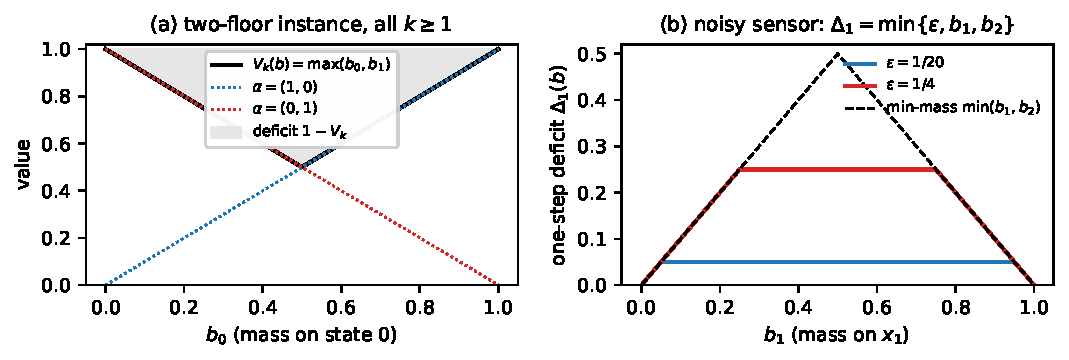
\includegraphics[width=\linewidth]{fig1_deficits.pdf}
\caption{Deficits attained and deficits below the minimal mass. (a) The two-floor instance: the value is $\max(b_0,b_1)$ for every horizon, the two witnesses $(1,0)$ and $(0,1)$ are the indicators of the two maximal survivable singletons, and the shaded deficit equals the minimal mass at every prior. (b) The two-state noisy sensor of Proposition~\ref{prop:pathdeficit}: the optimized one-step deficit is $\min\{\varepsilon,b_1,b_2\}$, which falls strictly below the minimal mass (dashed) on the whole interior plateau; at $b=(\tfr12,\tfr12)$ and $\varepsilon=\tfr1{20}$ the deficit is $\tfr1{20}$ against a minimal mass of $\tfr12$.}
\label{fig:deficits}
\end{figure}
\section{The delayed hidden-regime class: closed forms and the class lattice}\label{sec:delayed}

\subsection{The instance}

A scalar state $z$ measures the distance above a floor, the safe set being $\{z\ge1\}$. A hidden regime $\theta\in\{-1,+1\}$, with prior mass $w\in[0,1]\cap\Qr$ on $\theta=+1$, gates the effect of a binary control $u_t\in\{-1,+1\}$:
\begin{equation}\label{eq:delayed}
z_{t+1}=z_t+\theta\,u_t .
\end{equation}
No observation other than the exit announcement arrives before stage $\Tobs\ge1$, at which $\theta$ is revealed exactly. The prior places mass $w$ and $1-w$ on the two branches $(z_0,+1)$ and $(z_0,-1)$; under a segment $u$ the $\theta=+1$ branch sits at $z_0+\sum_t u_t$ and the $\theta=-1$ branch at $z_0-\sum_t u_t$, so the support follows two mirror-image trajectories. From a fixed $z_0$ only the states $z_0+j$, $|j|\le k$, are reachable within $k$ stages, so the reachable model is a finite safety POMDP in the sense of Definition~\ref{def:model}, with deterministic kernels and observation maps. The instance is the delayed-observation instance of the calculus \cite{Abaee2026calc}: its \emph{timing certificate} asserts nonviability of the hold-until-review regulator exactly when $\Tobs$ exceeds the exit time $\sigma^{*}=z_0-1$ of the falling branch, i.e.\ when $z_0<1+\Tobs$.

The effective window at horizon $k$ is $\ell=\min(k,\Tobs)$: after revelation the controller plays the rising control $u=\theta$ and never exits, so survival to horizon $k$ is survival of the first $\ell$ stages.

\subsection{Closed forms}

\begin{theorem}[parametric closed forms]\label{thm:closed}
On the instance \eqref{eq:delayed}, for every $z_0\in\R$, every rational $w\in[0,1]$, every $\Tobs\ge1$ and every horizon $k\ge1$ with $\ell=\min(k,\Tobs)$,
\begin{align}
V^{\hold}_k(b_0)&=\begin{cases}0,&z_0<1,\\ 1,&z_0\ge1+\ell,\\ \max(w,1-w),&1\le z_0<1+\ell,\end{cases}\label{eq:hold}\\[2pt]
V^{\ol}_k(b_0)=V^{\seq}_k(b_0)&=\begin{cases}0,&z_0<1,\\ 1,&z_0\ge2,\\ \max(w,1-w),&1\le z_0<2,\end{cases}\label{eq:ol}\\[2pt]
V^{\obs}_k(b_0)&=\ind{z_0\ge1},\label{eq:obs}
\end{align}
and $V_0(b_0)=\ind{z_0\ge1}$ for every class. The value-one region of the hold class is $z_0\ge1+\ell$; at and after revelation its boundary is $1+\Tobs$, the locus of the timing certificate.
\end{theorem}

\begin{proof}
Survival requires $z_0\ge1$ at stage $0$, so all values vanish for $z_0<1$. \emph{Hold class.} Under the hold $u\equiv+1$ the $\theta=+1$ branch rises and is safe, while the $\theta=-1$ branch sits at $z_0-t$ at stage $t$ and survives the window exactly when $z_0-\ell\ge1$; the surviving mass is $w+(1-w)\ind{z_0\ge1+\ell}$. The hold $u\equiv-1$ is the mirror image, with surviving mass $(1-w)+w\ind{z_0\ge1+\ell}$. Maximizing over the two holds gives \eqref{eq:hold}. \emph{Open-loop class.} Whatever the first move, one branch is sent to $z_0-1$, so joint survival requires $z_0\ge2$; conversely the alternating segment $(+1,-1,+1,\dots)$ has partial sums in $\{0,1\}$, keeps both branches in $[z_0-1,z_0+1]$, and is safe whenever $z_0\ge2$. A single branch is kept alive by the constant segment that makes it rise, so off the joint region the value is the larger prior mass. \emph{Sequential class.} Inside the window the only observation is the exit announcement. On the event that both branches survive, the two histories coincide (``no exit'' at every stage), so a sequential policy plays the same segment on both branches and the joint-survival condition is the open-loop one; a single branch is already savable open-loop. Hence $V^{\seq}_k=V^{\ol}_k$. \emph{Observed class.} With $\theta$ known at stage $0$ the control $u=\theta$ makes every branch rise from $z_0\ge1$.
\end{proof}

\begin{figure}[t]
\centering
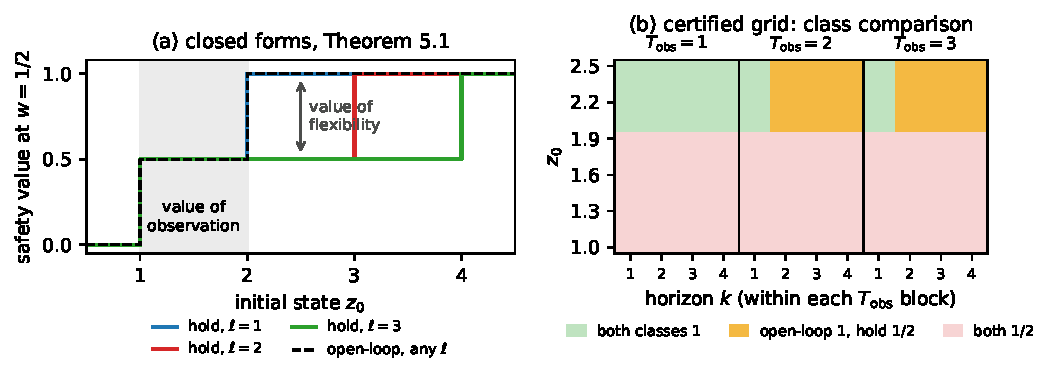
\includegraphics[width=\linewidth]{fig2_closedforms.pdf}
\caption{The delayed hidden-regime class. (a) Closed forms of Theorem~\ref{thm:closed} at the symmetric prior: the hold-class value jumps from $0$ to $\tfr12$ at $z_0=1$ and from $\tfr12$ to $1$ at $z_0=1+\ell$, $\ell=\min(k,\Tobs)$; the open-loop value (dashed, coinciding with the hold value for $\ell=1$) jumps to $1$ at $z_0=2$. The shaded band $[1,2)$ is where the value of observation is $\tfr12$; the vertical arrow marks the value of flexibility on $[2,1+\ell)$. (b) The certified grid ($z_0\in\{1.0,\dots,2.5\}$, $\Tobs\in\{1,2,3\}$, $k\in\{1,\dots,4\}$): green cells have value one in both classes, orange cells are the $36$ cell--horizon combinations on which open-loop time variation lifts the hold-class value $\tfr12$ to one (Corollary~\ref{cor:timing}), pink cells have value $\tfr12$ in both classes.}
\label{fig:closed}
\end{figure}

\subsection{The class lattice and its realized gaps}

\begin{theorem}[class lattice]\label{thm:lattice}
For the value of Definition~\ref{def:value}, $\Pi\subseteq\Pi'$ implies $V^{\Pi}_k\le V^{\Pi'}_k$. On the instance \eqref{eq:delayed}, for $k\ge1$, $\ell=\min(k,\Tobs)$ and $z_0\ge1$,
\[
V^{\hold}_k\ \le\ V^{\ol}_k\ =\ V^{\seq}_k\ \le\ V^{\obs}_k ,
\]
and both gaps are realized exactly on disjoint cells:
\begin{align}
V^{\ol}_k(b_0)-V^{\hold}_k(b_0)&=\min(w,1-w)\cdot\ind{2\le z_0<1+\ell}\qquad\text{(the value of flexibility)},\label{eq:flex}\\
V^{\obs}_k(b_0)-V^{\ol}_k(b_0)&=\min(w,1-w)\cdot\ind{1\le z_0<2}\qquad\ \ \text{(the value of observation)}.\label{eq:voi2}
\end{align}
At the symmetric prior each gap equals $\tfr12$ on its cells and $0$ elsewhere.
\end{theorem}

\begin{proof}
Monotonicity in the class is immediate from the maximizing definition, and the chain is $\Pi_{\hold}(\ell)\subseteq\Pi_{\ol}(\ell)\subseteq\Pi_{\seq}$ together with the information refinement defining $\Pi_{\obs}$. The middle equality is part of Theorem~\ref{thm:closed}. Subtracting the case displays \eqref{eq:hold}--\eqref{eq:obs}: the hold and open-loop forms differ exactly where $2\le z_0<1+\ell$, by $1-\max(w,1-w)=\min(w,1-w)$; the open-loop and observed forms differ exactly where $1\le z_0<2$, by the same amount. The two regions are disjoint.
\end{proof}

\begin{corollary}[the timing obstruction is class-scoped]\label{cor:timing}
The hold class and the sequential class coincide at the one-step horizon. For $k\ge2$ they differ exactly on $\{2\le z_0<1+\min(k,\Tobs)\}$, where an alternating open-loop segment keeps both branches at or above the floor while no constant hold does. In particular, the timing certificate of the calculus---firing exactly when $z_0<1+\Tobs$---is exact for the hold class at every horizon $k>\Tobs$ and over-fires relative to the sequential class exactly on $\{2\le z_0<1+\Tobs\}$; it certifies nonviability \emph{within the declared hold-until-review class}, and nothing more. On the certified grid of Figure~\ref{fig:closed}b the difference set consists of the $12$ timing cells $(\Tobs\in\{2,3\},\ z_0\in\{2.0,\dots,2.5\})$ at each of $k=2,3,4$, i.e.\ $36$ cell--horizon combinations.
\end{corollary}

\begin{proof}
At $k=1$ both classes choose one blind action. For $k\ge2$ the difference set is \eqref{eq:flex}; the alternating segment and the falling-branch exit at $z_0-\ell<1$ are the two mechanisms named in the proof of Theorem~\ref{thm:closed}. On the grid, $1+\min(k,\Tobs)\ge3>2.5$ for $k\ge2$ and $\Tobs\ge2$, so the difference set is $\{z_0\ge2\}\times\{\Tobs\ge2\}\times\{k\ge2\}$, of size $6\times2\times3=36$; for $\Tobs=1$ the set $\{2\le z_0<2\}$ is empty.
\end{proof}

\begin{remark}[reading the declaration]\label{rem:declaration}
The class declaration is part of the model, not a defect of the certificate. A regulator who sets a harvest rule and reviews it only at the end of a reporting window is the hold class; one who may pre-commit to a time-varying schedule is the open-loop class; one who receives the regime report early is the observed class. Theorem~\ref{thm:lattice} prices the three institutional designs on the same instance and separates two distinct levers: flexibility within a blind window buys $\min(w,1-w)$ on the timing cells, and earlier observation buys the same amount on the common-action cells, where no blind schedule can help. The word ``adaptive'' is avoided for blind windows: while no observation arrives, the only available distinction is between constant and time-varying open-loop control.
\end{remark}

\subsection{The certified grid}

The calculus certifies the instance on the grid $z_0\in\{1.0,1.1,\dots,2.5\}$, $\Tobs\in\{1,2,3\}$ (48 cells) at horizons $k\le4$ and the symmetric prior. Theorem~\ref{thm:closed} turns the certified records into corollaries.

\begin{corollary}[the certified grid]\label{cor:grid}
On the certified grid at $w=\tfr12$:
\begin{enumerate}[leftmargin=1.6em,itemsep=1pt]
\item[(a)] the hold-class value is $1$ exactly when $z_0\ge1+\min(k,\Tobs)$ and $\tfr12$ otherwise: $36$ unit values and $156$ half values among the $192$ cell--horizon combinations (Table~S1.1), and the segment-form enumeration of the class returns the closed form on every combination;
\item[(b)] the two hold-direction witnesses per combination give $384$ exact vectors of three types, $(1,1)$ with $72$ occurrences and the mirror pair $(1,0)$, $(0,1)$ with $156$ occurrences each; after exact deduplication $348$ distinct vectors remain, one per unit-value combination and two per half-value combination---the three-type census is the antichain of Theorem~\ref{thm:antichain} read off the grid, the maximal survivable sets being $\{+,-\}$ when $z_0\ge1+\ell$ and the two singletons otherwise;
\item[(c)] the certificate partition coincides with the value boundaries: $6$ viable cells ($V_k\equiv1$), $30$ common-action cells ($V_1<1$), $12$ timing cells ($V_1=1$, $V_{\Tobs+1}<1$);
\item[(d)] as a function of $z_0$ the hold-class value has exactly two jump loci, $z_0=1$ (from $0$ to $\tfr12$) and $z_0=1+\min(k,\Tobs)$ (from $\tfr12$ to $1$), the witness family changing at the same loci (Section~S3);
\item[(e)] on the $42$ nonviable cells the hold-class deficit is $\tfr12$ at every horizon with $k>z_0-1$ and $0$ before: on the timing cells $0$ at $k=1$ and $\tfr12$ at $k\ge2$, on the common-action cells $\tfr12$ at every $k\ge1$---the minimal-mass bound attained from the first horizon at which the falling branch exits.
\end{enumerate}
\end{corollary}

\begin{proof}
All items are the case analysis of \eqref{eq:hold} on the grid; the counts are enumerated by the verification script (Section~\ref{sec:verification}). For (a), $z_0\ge1+\ell$ on the grid forces $\ell=1$, i.e.\ $k=1$ or $\Tobs=1$, and $z_0\ge2$: $6$ states $\times$ ($4$ horizons at $\Tobs=1$, plus $k=1$ at $\Tobs=2,3$) $=36$. For (b), each unit-value combination has both witnesses equal to $(1,1)$, so $2\times36=72$ coincide; the remaining $156$ combinations contribute the mirror pair. For (c), $V_1<1$ iff $z_0<2$ ($10$ states $\times3$ windows), and $V_{\Tobs+1}<1$ with $V_1=1$ iff $2\le z_0<1+\Tobs$ ($6$ states at $\Tobs=2,3$).
\end{proof}
\section{Late information: learning deadlines and their exact price}\label{sec:deadline}

Observation is a design variable. In the delayed instance the regime is revealed exogenously; in many sustainability settings---an unknown regeneration rate, an uncertain climate sensitivity, an institution whose effectiveness is unknown---the hidden parameter can only be learned by acting, and acting on a wrong hypothesis is costly. This section prices that structure exactly on a second instance and then states the general threshold law behind it.

\subsection{The declining instance}

A stock $z$ drifts down by $\tfr1{10}$ per stage unless corrected; the correction is gated by a hidden sign $\theta\in\{-1,+1\}$:
\begin{equation}\label{eq:declining}
z_{t+1}=z_t-\tfr1{10}+\theta\,u_t,\qquad u_t\in\{-1,0,+1\},\qquad\text{safe set }\{z\ge1\}.
\end{equation}
Holding $u=0$ is blind: the displacement $-\tfr1{10}$ is the same on both branches. Any $u\neq0$ is a \emph{probe}: the displacement $-\tfr1{10}\pm1$ separates the branches by $2$, so a single reading of the displacement reveals $\theta$ exactly and the posterior collapses---one observation splits the belief with no statistics. The \emph{learned} control $u=\theta$ has drift $-\tfr1{10}+\theta^{2}=\tfr9{10}>0$ and is safe forever from any $z\ge1$; the wrong control $u=-\theta$ has drift $-\tfr{11}{10}$.

\begin{proposition}[probes and learning deadlines]\label{prop:deadline}
On the instance \eqref{eq:declining} with the grid $z_0\in\{1.0,\dots,2.5\}$:
\begin{enumerate}[leftmargin=1.6em,itemsep=1pt]
\item[(a)] with $\theta$ observed from the start every $z_0\ge1$ is viable ($16$ of $16$ grid states);
\item[(b)] with a free probe (probe at stage $0$, then the learned control) viability holds exactly when $z_0\ge\tfr{21}{10}$, independently of any deadline ($5$ grid states);
\item[(c)] in the \emph{pinned-probe family}---hold $u=0$ to the deadline $\Tl$, probe at $\Tl$, then the learned control, no earlier probe being admissible---viability holds exactly when
\begin{equation}\label{eq:deadline}
z_0\ \ge\ \tfr{21}{10}+\tfr{\Tl}{10},\qquad \Tl=0,1,2,\dots,
\end{equation}
so the viable set on the grid shrinks linearly and antitonically in the deadline, $|K|=5,4,3,2,1$ for $\Tl=0,\dots,4$;
\item[(d)] with probe-free exogenous revelation at $\Tl$ (hold $u=0$, then the learned control) viability holds exactly when $z_0\ge1+\tfr{\Tl}{10}$, with $|K|=16,15,14,13,12$ for $\Tl=0,\dots,4$.
\end{enumerate}
The pinned family sits between the two benchmarks: the flat free-probe threshold prices the probe excursion alone, the probe-free threshold prices the blind decline alone, and \eqref{eq:deadline} prices both (Figure~\ref{fig:deadlines}, Table~S4.1).
\end{proposition}

\begin{proof}
(a) $u=\theta$ from $z_0\ge1$ never exits. (b) The probe moves the branches to $z_0-\tfr1{10}\pm1$; the $\theta=-1$ branch requires $z_0-\tfr{11}{10}\ge1$. (c) Before the deadline the state falls to $z_0-\tfr{\Tl}{10}$, which must stay at or above the floor; the probe then requires $z_0-\tfr{\Tl}{10}-\tfr{11}{10}\ge1$, the binding condition; afterwards the learned control is safe. The branch positions after the probe differ by $2$, so the reading identifies $\theta$. The grid counts follow from \eqref{eq:deadline}. (d) Only the blind decline must be survived: $z_0-\tfr{\Tl}{10}\ge1$.
\end{proof}

\begin{figure}[t]
\centering
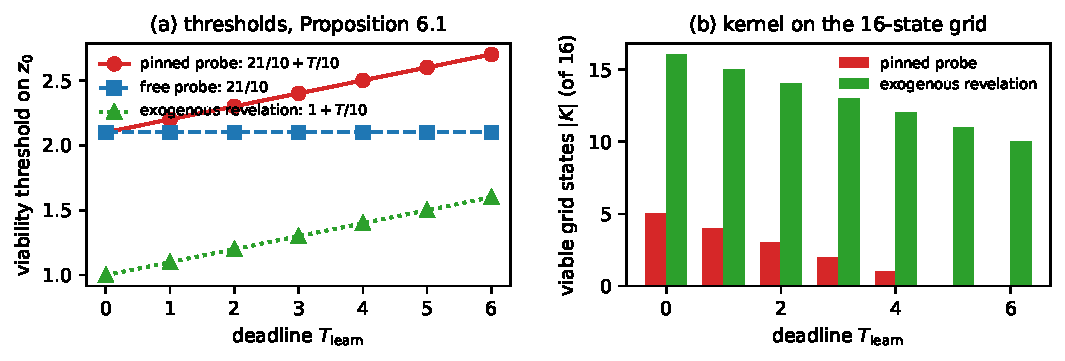
\includegraphics[width=\linewidth]{fig3_deadlines.pdf}
\caption{Learning deadlines on the declining instance. (a) The pinned-probe threshold $\tfr{21}{10}+\tfr{\Tl}{10}$ of Proposition~\ref{prop:deadline} between the flat free-probe benchmark $\tfr{21}{10}$ and the probe-free benchmark $1+\tfr{\Tl}{10}$. (b) Viable grid states: $5,4,3,2,1$ for the pinned probe and $16,\dots,12$ for exogenous revelation at $\Tl=0,\dots,4$; beyond $\Tl=4$ the pinned family is empty on the grid. The grid counts form a staircase, not a continuous law; the thresholds are exact for every real $z_0$.}
\label{fig:deadlines}
\end{figure}

\subsection{The general schedule law}

\begin{theorem}[exact threshold of a hold--probe--learn schedule]\label{thm:additive}
Let the hidden parameter $\theta$ range over a finite set $\Theta$ and enter the drift additively, $z_{t+1}=z_t+d(u_t,\theta)$, with floor $z\ge1$. Consider the schedule: hold $u_0$ for $T\ge0$ stages, probe with $u_p$ for one stage (the displacement $d(u_p,\cdot)$ being injective on $\Theta$, so the probe reveals $\theta$), then play $u^{*}(\theta)$ with $\mu=\min_{\theta}d(u^{*}(\theta),\theta)>0$. Then the schedule is viable for every horizon if and only if
\begin{equation}\label{eq:general}
z_0\ \ge\ 1+\max_{\theta\in\Theta}\max\bigl\{0,\ -T\,d(u_0,\theta),\ -T\,d(u_0,\theta)-d(u_p,\theta)\bigr\}.
\end{equation}
Let $d_0=\max_\theta(-d(u_0,\theta))\ge0$ be the worst hold loss and $e_p=\max_\theta(-d(u_p,\theta))\ge0$ the worst probe excursion. If some $\theta^{*}$ attains both maxima (\emph{aligned worst losses}), \eqref{eq:general} is the additive law
\begin{equation}\label{eq:additive}
z_0\ \ge\ 1+T\,d_0+e_p .
\end{equation}
Without alignment the additive right-hand side is only an upper bound on the exact threshold, and the gap can be positive.
\end{theorem}

\begin{proof}
On each branch $\theta$ the path is linear within each phase, so its minimum over the hold--probe prefix is attained at a phase endpoint: at $z_0$, at $z_0+T\,d(u_0,\theta)$, or at $z_0+T\,d(u_0,\theta)+d(u_p,\theta)$; after the probe the learned drift $\mu>0$ lifts the state away from the floor forever. Viability on every branch is therefore the conjunction of the three endpoint conditions over $\theta$, which is \eqref{eq:general}. Under alignment the third term at $\theta^{*}$ equals $T d_0+e_p$, which dominates the other terms because $d_0,e_p\ge0$, giving \eqref{eq:additive}; in general $\max_\theta(-Td(u_0,\theta)-d(u_p,\theta))\le Td_0+e_p$, with strict inequality possible.
\end{proof}

\begin{example}[two aligned instances and a misaligned one]\label{ex:additive}
The declining instance has $d_0=\tfr1{10}$ (attained at both $\theta$) and $e_p=\tfr{11}{10}$ (attained at $\theta=-1$), so the losses are aligned and \eqref{eq:additive} is \eqref{eq:deadline}. A second instance, $z_{t+1}=z_t-\tfr3{20}+\tfr9{10}\,\theta u_t$, has $d_0=\tfr3{20}$ and $e_p=\tfr{21}{20}$ and threshold $\tfr{41}{20}+\tfr{3T}{20}$; both are verified by exact enumeration for all swept $(z_0,T)$. Alignment is essential: with $\Theta=\{-1,+1\}$, hold drift $d(u_0,\theta)=-\tfr12+\tfr12\theta$, probe drift $d(u_p,\theta)=-\tfr12-\tfr12\theta$ and learned drift $1$, the worst hold loss $d_0=1$ is attained at $\theta=-1$ and the worst probe excursion $e_p=1$ at $\theta=+1$; the additive right-hand side at $T=1$ is $3$, but \eqref{eq:general} gives the exact threshold $2$, and indeed from $z_0=2$ both branches follow the paths $(2,1,1)$ and $(2,2,1)$ and then rise.
\end{example}

\begin{remark}[the delayed instance as a schedule]\label{rem:delayedschedule}
The delayed instance of Section~\ref{sec:delayed} under the hold class is the schedule of Theorem~\ref{thm:additive} with $T=\Tobs$, no probe ($e_p=0$), hold loss $d_0=1$ on the falling branch and the learned control $u=\theta$ afterwards: \eqref{eq:additive} gives $z_0\ge1+\Tobs$, the locus of the timing certificate and of the value-one boundary of \eqref{eq:hold} at $k>\Tobs$. The same law therefore prices exogenous and endogenous revelation on one scale: a unit of blind decline per stage, plus the excursion of whatever experiment produces the information.
\end{remark}
\section{The stochastic layer: noisy sensing}\label{sec:stochastic}

Everything so far has deterministic kernels and observation maps; the values are prior masses of surviving branches and take finitely many values dictated by the prior. This section opens the stochastic layer, where the values cease to be prior masses and the minimal-mass bound ceases to be universal.

\subsection{The weighted-path identity}

For a fixed policy $\pi$ the exit probability from the belief $b$ is linear in $b$: $\Prob_\pi(\text{exit by stage }k\mid b)=\sum_x b(x)\,q^{\pi}_k(x)$, with $q^{\pi}_k(x)$ the exit probability from the initial state $x$. The deficit is therefore the prior mass weighted by \emph{fatal-path probabilities} under the optimal policy; under deterministic kernels $q^{\pi}_k\in\{0,1\}$ and the identity collapses to the survived-mass formula. The one-step read-then-act case already separates the two layers.

\begin{proposition}[weighted-path deficit and the sensor instance]\label{prop:pathdeficit}
Let a reading $y$ of the initial state be available before the first action, with a normalized law $g_0(y\mid x)$, and let the controller choose $a=a(y)$. Then
\begin{equation}\label{eq:pathdeficit}
\Delta_1(b)=\min_{a(\cdot)}\ \sum_{x}b(x)\,p^{a(\cdot)}_x,\qquad p^{a(\cdot)}_x=\sum_y g_0(y\mid x)\,p(x,a(y)),
\end{equation}
the minimum over deterministic reading-to-action maps; randomization cannot lower it. In the two-state sensor instance---safe states $x_1,x_2$, action $a_i$ safe only at $x_i$, reading error $\Prob(\text{reads }j\neq i\mid x_i)=\varepsilon$ with $0<\varepsilon<\tfr12$---the four maps give the deficits $\varepsilon$ (read-own), $1-\varepsilon$ (read-opposite), $b(x_2)$ (always $a_1$) and $b(x_1)$ (always $a_2$), so
\begin{equation}\label{eq:sensor}
\Delta_1(b)=\min\{\varepsilon,\ b(x_1),\ b(x_2)\}.
\end{equation}
At $b=(\tfr12,\tfr12)$ and $\varepsilon=\tfr1{20}$ the deficit is $\tfr1{20}$, strictly below the minimal mass $\tfr12$ (Figure~\ref{fig:deficits}b).
\end{proposition}

\begin{proof}
For a fixed map, one-step survival is $\sum_x b(x)\sum_y g_0(y\mid x)(1-p(x,a(y)))$, which is \eqref{eq:pathdeficit} after optimizing; a randomized map is a convex combination of deterministic ones and the objective is linear in it. In the sensor instance the four maps are enumerated directly; for $\varepsilon<\tfr12$ the read-opposite map is never optimal, giving \eqref{eq:sensor}.
\end{proof}

The identity delimits the reach of the deterministic layer. The minimal-mass bound \eqref{eq:minmass} requires every admissible policy to lose some whole branch of positive prior mass; with noisy readings an optimal policy loses an $\varepsilon$-fraction of \emph{every} branch and no branch entirely, and the deficit can be far below the smallest prior mass. The calculus's probabilistic development, in which the deficit from unity is bounded below by the smallest compatible mass under adversarial disturbance readings, is exact at the deterministic degeneration of Remark~\ref{rem:operators} and is scoped to it.

\subsection{Noisy probes and the repetition trade-off}

\begin{proposition}[noisy probe and majority reading]\label{prop:noisyprobe}
On the declining instance \eqref{eq:declining}, hold $u=0$ to stage $t_p$, take at stage $t_p$ an instantaneous reading of $\theta$ that is correct with probability $1-\varepsilon$ and flipped with probability $\varepsilon$, and play $u=$ reading from $t_p$ to the horizon $k\ge t_p$. With $z_p=z_0-\tfr{t_p}{10}$,
\begin{equation}\label{eq:noisyprobe}
V_k(b_0)=(1-\varepsilon)\,\ind{z_p\ge1}+\varepsilon\,\ind{z_p\ge1+\tfr{11}{10}(k-t_p)} ,
\end{equation}
exactly: the correct reading acts under drift $\tfr9{10}$ and the flipped reading under drift $-\tfr{11}{10}$. The value takes exactly the three levels $\{0,1-\varepsilon,1\}$ and the deficit equals the post-reading minimal mass $\varepsilon$ precisely on the middle band $1\le z_p<1+\tfr{11}{10}(k-t_p)$. With three readings at $t_p,t_p+1,t_p+2$ ($u=0$ meanwhile) and a majority decision at $t_p+2$, the wrong-majority probability is
\begin{equation}\label{eq:majority3}
p_3=3\varepsilon^{2}(1-\varepsilon)+\varepsilon^{3}=\varepsilon^{2}(3-2\varepsilon),
\end{equation}
equal to $\tfr7{250}$ at $\varepsilon=\tfr1{10}$ against $\tfr1{10}$ for one reading, and \eqref{eq:noisyprobe} holds with $p_3$ in place of $\varepsilon$ and $z_0-\tfr{t_p+2}{10}$ in place of $z_p$: each additional reading costs $\tfr1{10}$ of floor margin to the blind drift---the exact exploration--safety exchange at this scale (Figure~\ref{fig:probes}a).
\end{proposition}

\begin{proof}
Condition on $(\theta,\text{reading})$, the four cases having probabilities $\tfr12(1-\varepsilon)$ and $\tfr12\varepsilon$ per branch. Before $t_p$ the state falls monotonically, so survival to $t_p$ is $z_p\ge1$. A correct reading then plays $u=\theta$, with drift $\tfr9{10}$, and never exits; a flipped reading plays $u=-\theta$, with drift $-\tfr1{10}-1=-\tfr{11}{10}$, and survives to $k$ exactly when $z_p-\tfr{11}{10}(k-t_p)\ge1$. Summing gives \eqref{eq:noisyprobe}; both branches contribute symmetrically, so the prior weight does not appear. The wrong-majority event is two or three flipped readings, with probability \eqref{eq:majority3}; the two extra blind stages lower the state by $\tfr2{10}$ before the decision. Both displays are re-derived by exhaustive enumeration over $(\theta,\text{readings})$ in the verification script.
\end{proof}

\begin{proposition}[probe-count bound]\label{prop:probecount}
Let $n=2m+1$ readings with per-reading error $\varepsilon<\tfr12$ be decided by majority. Then
\begin{equation}\label{eq:probecount}
p_{\mathrm{wrong}}(n)=\sum_{j=m+1}^{n}\binom nj\varepsilon^{j}(1-\varepsilon)^{n-j}\ \le\ \bigl(4\varepsilon(1-\varepsilon)\bigr)^{n/2}\ \le\ e^{-2n\,\mathrm{sep}^{2}},\qquad \mathrm{sep}=\tfr12-\varepsilon,
\end{equation}
so $n\ge\ln(1/\delta)/(2\,\mathrm{sep}^{2})$ readings achieve a wrong-majority probability at most $\delta$: the reading count grows like $\log(1/\delta)$ over the squared separation, and on the declining instance each reading costs $\tfr1{10}$ of floor margin. At $\varepsilon=\tfr1{10}$ the bound reads $(3/5)^{n}$, against the exact values $\tfr1{10},\tfr7{250},\tfr{107}{12500},\tfr{341}{125000},\tfr{22273}{25000000}$ at $n=1,3,5,7,9$ (Figure~\ref{fig:probes}b, Table~S5.1).
\end{proposition}

\begin{proof}
For $j>n/2$, $\varepsilon^{j}(1-\varepsilon)^{n-j}=(\varepsilon(1-\varepsilon))^{n/2}\bigl(\tfrac{\varepsilon}{1-\varepsilon}\bigr)^{j-n/2}\le(\varepsilon(1-\varepsilon))^{n/2}$ because $\varepsilon<1-\varepsilon$; summing the binomial coefficients over all $j$ bounds the sum by $2^{n}(\varepsilon(1-\varepsilon))^{n/2}$, which is the first inequality. The second is $4\varepsilon(1-\varepsilon)=1-4\,\mathrm{sep}^{2}\le e^{-4\,\mathrm{sep}^{2}}$ \cite{Hoeffding1963}.
\end{proof}

\begin{remark}[noiseless limit]\label{rem:eps0}
The exact split of Proposition~\ref{prop:deadline} is the $\varepsilon\to0$ degeneration of Proposition~\ref{prop:probecount}: the separation rises to $\tfr12$, $p_{\mathrm{wrong}}(1)=\varepsilon$ falls to zero, and one reading already achieves $\delta=0$---the branch split of size $2$ needs no statistics precisely because the base of the exponential tends to zero with $\varepsilon$. For $\varepsilon>0$ the count law prices what the exact split obtains for free, and each reading additionally pays its unit of floor margin.
\end{remark}

\begin{figure}[t]
\centering
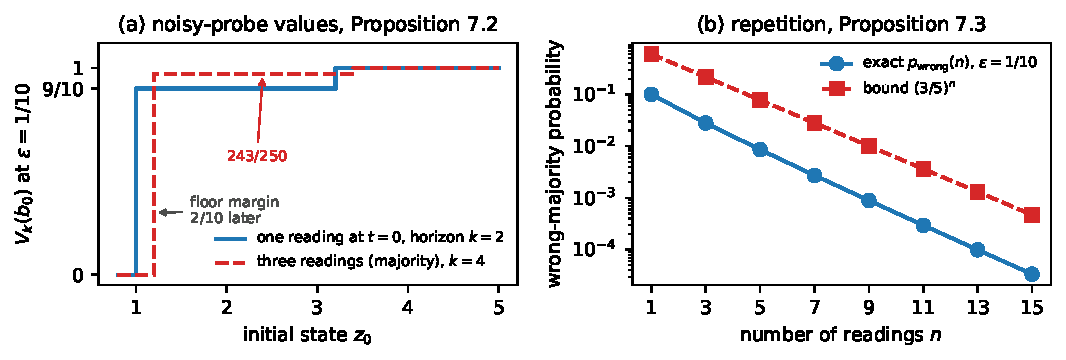
\includegraphics[width=\linewidth]{fig4_probes.pdf}
\caption{Noisy probes on the declining instance. (a) Values of Proposition~\ref{prop:noisyprobe} at $\varepsilon=\tfr1{10}$ with a single reading at $t_p=0$ and horizon $k=2$ (three levels $0,\tfr9{10},1$ with jumps at $z_0=1$ and $z_0=1+\tfr{11}{10}\cdot2$), and with three readings decided by majority at stage $2$ and horizon $k=4$ (levels $0,\tfr{243}{250},1$, both jumps shifted right by the $\tfr2{10}$ of floor margin spent on the two extra blind stages). (b) The exact wrong-majority probability against the bound $(3/5)^{n}$ of Proposition~\ref{prop:probecount}.}
\label{fig:probes}
\end{figure}
\section{Between expectation and worst case: contamination ambiguity}\label{sec:dr}

Remark~\ref{rem:operators} supplies two endpoints: the expected operator \eqref{eq:recursion} and the adversarial reading of the observation. A contamination ambiguity set \cite{Huber1964} interpolates between them. Fix a nominal law $p$ on the outcomes of a stage and the set
\[
\calD_\rho(p)=\{\,q=(1-\rho)\,p+\rho\,r:\ r\in\Delta(Y^{\bot})\,\},\qquad \rho\in[0,1],
\]
and define the contaminated recursion $V^{\rho}_0(b)=b(\calV)$,
\begin{equation}\label{eq:rho}
V^{\rho}_{k+1}(b)=\max_{a}\ \inf_{q\in\calD_\rho(\Prob(\cdot\mid b,a))}\ \sum_{y\in Y^{\bot}}q(y)\,V^{\rho}_k\bigl(\tau(b,a,y)\bigr),
\end{equation}
with $V^{\rho}_k(\delta_\bot)=0$. The operator needs a continuation at \emph{every} outcome on which contamination may concentrate; outcomes that are nominally null must either be removed from the contaminating support or be given an explicit off-support continuation, and the construction---fixing the nominal posteriors while perturbing the outcome probabilities---is a rectangular stress operator in the sense of robust Markov decision processes \cite{Iyengar2005,NilimElGhaoui2005}, not the Bayesian update of a single coherent perturbed joint law.

\begin{proposition}[one-stage contamination and its limits]\label{prop:dr}
\begin{enumerate}[leftmargin=1.6em,itemsep=1pt]
\item[(i)] The inner infimum in \eqref{eq:rho} is exact: for continuation values $(v_y)$,
\begin{equation}\label{eq:contam}
\inf_{q\in\calD_\rho(p)}\sum_y q(y)\,v_y=(1-\rho)\sum_y p(y)\,v_y+\rho\,\min_y v_y ,
\end{equation}
the adversary spending the whole budget on the worst outcome; $\rho=0$ recovers the expected operator and $\rho=1$ the worst-case reading.
\item[(ii)] The interpolation is not affine across stages: with one safe state $s$, one action, $T(s\mid s)=\tfr12$, and an observation that reveals survival or exit, the recursion gives $V^{\rho}_k(\delta_s)=\bigl(\tfr{1-\rho}2\bigr)^{k}$, so $V^{1/2}_2=\tfr1{16}$ while $(1-\rho)V^{0}_2+\rho V^{1}_2=\tfr18$ at $\rho=\tfr12$.
\item[(iii)] $V^{\rho}_k$ is piecewise linear in $b$ for every $\rho$, convex at $\rho=0$ (Proposition~\ref{prop:alpha}), and in general not convex for $\rho>0$, the minimum in \eqref{eq:contam} being a concave operation; no concavity holds either, the two-floor value $\max(b_0,b_1)$ at $\rho=0$ being a counterexample.
\end{enumerate}
\end{proposition}

\begin{proof}
(i) The objective is linear in $r$ over the simplex, so the infimum is attained at a vertex $r=\delta_{y^{*}}$ with $y^{*}$ a minimizer of $v_y$. (ii) $V^{\rho}_1(\delta_s)=(1-\rho)\bigl(\tfr12\cdot1+\tfr12\cdot0\bigr)+\rho\cdot0=\tfr{1-\rho}2$, and the same step applied to the continuation $V^{\rho}_{k}(\delta_s)$ gives the product form; the endpoint values are $V^{0}_2=\tfr14$ and $V^{1}_2=0$. (iii) Piecewise linearity: \eqref{eq:contam} is a maximum over actions of a sum of piecewise linear functions and a pointwise minimum of piecewise linear functions; convexity fails because the minimum of convex functions need not be convex, and concavity fails already at $\rho=0$.
\end{proof}

\begin{proposition}[prior contamination on the delayed class]\label{prop:priorcontam}
On the instance \eqref{eq:delayed} let the prior itself be contaminated, $q(+1)=(1-\rho)w+\rho r$ with $r\in[0,1]$ chosen adversarially after the hold is announced. Then, for $k\ge1$ and $\ell=\min(k,\Tobs)$,
\begin{equation}\label{eq:priorcontam}
V^{\rho,\hold}_k(b_0)=\begin{cases}0,&z_0<1,\\ 1,&z_0\ge1+\ell,\\ (1-\rho)\max(w,1-w),&1\le z_0<1+\ell,\end{cases}
\end{equation}
the adversary pouring the contamination onto the falling branch; at the symmetric prior the three levels are $0$, $\tfr{1-\rho}2$ and $1$.
\end{proposition}

\begin{proof}
Off the middle band the hold saves nothing or everything regardless of the prior. On the band the hold $u\equiv+1$ saves the $\theta=+1$ branch, of contaminated mass $(1-\rho)w+\rho r$, minimized at $r=0$; the hold $u\equiv-1$ saves the other branch, of mass $(1-\rho)(1-w)+\rho(1-r)$, minimized at $r=1$. The controller takes the better of $(1-\rho)w$ and $(1-\rho)(1-w)$.
\end{proof}

The contamination family is the formal home of the worst-case wording used informally across the companion papers: at $\rho=1$ the adversary chooses the observation, which under deterministic kernels is the robust operator of Remark~\ref{rem:operators}; at $\rho=0$ the nominal law is trusted. Moment- and distance-based ambiguity sets over the transition or observation kernel \cite{Osogami2015,Nakao2021,Saghafian2018}, under which the value stays piecewise linear, are the natural next ring and are not developed here.
\section{Position among related work}\label{sec:related}

\paragraph{Belief-state reduction and $\alpha$-vectors.}
That a partially observed control problem can be rewritten as a fully observed one on the belief simplex is classical \cite{Astrom1965,BertsekasShreve1978}, and the finite-horizon value of a partially observable Markov decision process is piecewise linear and convex, represented by finitely many $\alpha$-vectors \cite{SmallwoodSondik1973,Monahan1982,Kaelbling1998}. The safety value is a belief-space value in that lineage with the multiplicative survival objective of probabilistic reachability \cite{Abate2008}, whose partially observed sufficient-statistic form is due to \cite{LesserOishi2014}. The present contribution is not the representation but what the representation becomes under deterministic kernels: an antichain of survival indicators (Theorem~\ref{thm:antichain}), computed exactly in rational arithmetic rather than in floating point, with the exact pruning of \cite{Cassandra1997} reduced to inclusion-maximality.

\paragraph{Viability under imperfect measurement.}
The closest work is the viability-theoretic treatment of imperfect information. Veliov \cite{Veliov1993} gives a \emph{sufficient} condition for the existence of an output-feedback regulation map, equivalent to Haddad's viability condition under perfect measurement; its failure is inconclusive. Luc Doyen \cite{Doyen2000}---the viability theorist, not Laurent Doyen of the qualitative partially observed literature cited below---gives \emph{necessary and sufficient} conditions for guaranteed viability of uncertain systems under state and control constraints, for Lipschitz memoryless closed loops $u(h(x,w))$ maintaining a closed domain exactly. Theorem~\ref{thm:support} sits between the two: it is necessary as well as sufficient, so its failure is informative; it admits history-dependent policies, and Proposition~\ref{prop:feedback} shows that the admission is strict and quantifies it; and its criterion is quantitative, near-misses being measured by the deficit rather than discarded. The estimation-space programme, which absorbs imperfect information into tubes of estimators for continuous-time differential games \cite{Cardaliaguet2007}, and the minimal-time-of-crisis measure of \cite{DoyenSaintPierre1997}, which quantifies constraint violation in time rather than in probability, are complementary and not competing. Stochastic viability under full observation \cite{DeLaraDoyen2008,DoyenDeLara2010} is the $\Pi_{\obs}$ benchmark of Theorem~\ref{thm:lattice}.

\paragraph{Qualitative analysis and verification of POMDPs.}
For almost-sure objectives the belief support is a sufficient statistic, and the decidability and complexity landscape of qualitative partially observable Markov decision processes is established \cite{Chatterjee2010,Chatterjee2016}; the support-based synthesis of almost-sure reachability controllers is pursued in \cite{Junges2021}, and probabilistic model checkers handle quantitative finite-horizon POMDP properties by grid and point-based methods \cite{Norman2017,Bouton2020}. Theorem~\ref{thm:support} is the quantitative companion of the support reduction, and Proposition~\ref{prop:pathdeficit} shows where the reduction stops: under noisy sensing the deficit depends on the full belief, not on its support.

\paragraph{Complexity, robustness and learning.}
Finite-horizon partially observed problems are PSPACE-complete and their unobservable variant NP-complete \cite{PapadimitriouTsitsiklis1987}; bounds and point-based approximations are the standard response \cite{Lovejoy1991,Pineau2003}. This paper does not improve those results; it identifies classes on which exact answers are available in closed form and records where exactness stops. Robust Markov decision processes with rectangular ambiguity sets \cite{Iyengar2005,NilimElGhaoui2005} and their partially observed extensions \cite{Osogami2015,Nakao2021,Saghafian2018} are the formal setting of Section~\ref{sec:dr}; the contamination operator used here is the simplest member of that family and is chosen because its inner problem is exact. Shielding for learning agents \cite{Alshiekh2018} enforces safety for a learner with an unknown model; here the model is known and the question is exact sufficiency. The learning-deadline results of Section~\ref{sec:deadline} are not learning theory: they price, exactly, the state-space cost of acquiring one bit of structural information late.

\paragraph{What is claimed.}
Five things: exact sufficiency with a quantitative deficit (Theorem~\ref{thm:support}, Proposition~\ref{prop:deficit}); the survivable-set antichain with its attained Sperner bound and the attained value-of-observation bound (Theorem~\ref{thm:antichain}, Proposition~\ref{prop:feedback}); the parametric closed forms, the class lattice with its realized gaps and the class-scoping of the timing obstruction (Theorems~\ref{thm:closed} and~\ref{thm:lattice}, Corollary~\ref{cor:timing}); the exact price of late information (Proposition~\ref{prop:deadline}, Theorem~\ref{thm:additive}); and the stochastic layer with its identity, instances and bounds (Propositions~\ref{prop:pathdeficit}--\ref{prop:probecount}, \ref{prop:dr}--\ref{prop:priorcontam}). Not claimed: the belief-state reduction, the $\alpha$-vector representation as such, the qualitative complexity landscape, or the hardness results that motivate approximation.
\section{Exact verification and the machine-checked layer}\label{sec:verification}

\paragraph{Exact module and verification script.}
Every value, witness, threshold, count and tabulated entry in this paper is regenerated from the definitions by the exact module \texttt{p02\_core.py} and the verification script \path{paper02_probabilistic_sufficiency_v16_verification.py}, in integer and rational arithmetic with the Python standard library only, deterministically. The module implements a generic finite safety POMDP with the masked backup \eqref{eq:backup}, dominance pruning, open-loop enumeration and the contaminated operator \eqref{eq:rho}; the instances of the paper are built from it or enumerated directly from their dynamics. The script re-derives: the two-floor witnesses and values to horizon $5$ (Example~\ref{ex:twofloor}); the family $\mathcal F_n$ for $n=2,3,4$ with $V^{\seq}_2=1$ and $V^{\ol}_2=\max b$ (Proposition~\ref{prop:feedback}); the closed forms \eqref{eq:hold}--\eqref{eq:ol} against brute-force enumeration of all holds and all open-loop segments on a structured sweep of $(z_0,w,\ell)$ triples including $z_0<1$ and a seeded randomized battery; the $192$-combination grid, its $36/156$ census, the $384$ witnesses and their $348$ distinct vectors, the $6/30/12$ partition, the jump loci and the deficit profile (Corollary~\ref{cor:grid}); the identity of the class-difference set with $\{2\le z_0<1+\min(k,\Tobs)\}$ on an extended grid to $z_0=4.0$ and its $36$ combinations on the certified grid (Corollary~\ref{cor:timing}); the asymmetric audit (Example~\ref{ex:asym}); stabilization of both window classes to horizon $40$ (Proposition~\ref{prop:freeze}); the learning-deadline thresholds and kernel counts with both benchmarks (Proposition~\ref{prop:deadline}); the general schedule law on the two aligned instances and the misaligned example (Theorem~\ref{thm:additive}); the sensor deficits of all four maps on a prior sweep (Proposition~\ref{prop:pathdeficit}); the noisy-probe and majority closed forms against exhaustive enumeration over readings (Proposition~\ref{prop:noisyprobe}); the exact wrong-majority probabilities at $n=1,3,5,7,9$ against $(3/5)^{n}$ (Proposition~\ref{prop:probecount}); the contamination example and the prior-contamination closed form against vertex enumeration (Propositions~\ref{prop:dr}--\ref{prop:priorcontam}); and the two-patch instance of Section~S4. The script finally binds the headline numbers of the text to the recomputed values and checks the result numbers quoted in figure captions against the compiled auxiliary file. The record of the $62$ checks, all passing, is listed in Section~S7; the original campaign scripts of the earlier editions remain available in the repository and their verdicts are unchanged.

\paragraph{Machine-checked layer.}
Three combinatorial statements are formalized in Lean~4 \cite{deMouraUllrich2021} in the repository's \texttt{P3} modules: the support identity \eqref{eq:support} under its deterministic-kernel hypotheses together with the equivalence $V_k(b)=1\iff\supp b\in\Wfb_k$ on the feedback reading of Theorem~\ref{thm:support} (an earlier edition's blind reading is refuted there by an explicit counterexample, which is why the feedback/blind distinction of Proposition~\ref{prop:feedback} is stated as a result and not a remark); the freeze count and frozen value of Proposition~\ref{prop:freeze} for its specified action families; and the rationality and convexity of the $\alpha$-vectors of Proposition~\ref{prop:alpha}. The pinned project builds in continuous integration ($60/60$ jobs) with no \texttt{sorry}, \texttt{admit} or user axiom; three \texttt{native\_decide} uses in the support/value examples generate nine compiler-trust axiom names, which are executable computational certificates and are declared as such, not kernel-only proofs. One bound is cited rather than formalized: the Sperner bound of Theorem~\ref{thm:antichain}(iii). The general additive law, the noisy-probe formulas and the probe-count bound are verified by exact enumeration, not formalized. Details and provenance are in Section~S7.
\section{Discussion and conclusion}\label{sec:discussion}

\paragraph{What the value adds to the calculus.}
The set-valued theory asks whether an information state is viable; the safety value says how viable, and the two agree exactly where they should. On deterministic models the value-one level is the feedback viable-set recursion, the deficit is the lightest mass that any policy must abandon, the $\alpha$-vectors are the maximal survivable subsets, and the obstruction certificates are the deficit's lower-bound sides. The agreement is not merely qualitative: on the delayed hidden-regime class the certified table, census and witnesses are read off two closed forms, and the one place where the set-valued verdicts seemed to overreach---the timing certificate firing on cells where a time-varying schedule is safe---turns out to be a precise statement about the declared hold class. Two levers are separated and priced on the same instance: flexibility within a blind window and earlier observation each buy $\min(w,1-w)$, on disjoint cells. For a regulator the distinction is operational: on the timing cells a pre-committed alternating schedule is as good as early information, and on the common-action cells nothing but earlier information helps.

\paragraph{What the stochastic layer changes.}
With noisy sensing the deficit is a weighted sum of fatal-path probabilities, the minimal-mass bound is a statement about the deterministic limit, and the value becomes a design quantity for observation: a probe pinned to a deadline moves the viability threshold linearly in the deadline, a general schedule has an exact threshold which is additive exactly when the worst losses align, and repeated noisy readings purchase reliability at a fixed exchange rate in floor margin. These are small instances, but the laws are exact and the mechanisms---blind decline, probe excursion, wrong-action drift---are the ones that any larger model must contain.

\paragraph{Delimitations.}
The semantics is nominal expectation under a declared model; the robust quantifiers of the companion papers are recovered only at the deterministic degeneration, which is a change of operator, and the contamination family is where worst-case wording is given a formal home. Timing statements are class-scoped. No learning theory is claimed beyond the one-probe exact split and the majority count: Bayesian updating of continuous parameters, repeated experiments with design, and exploration--exploitation trade-offs are out of scope, and the hidden parameter enters additively. The $\alpha$-set growth is exponential in the worst case and the hardness results stand; the certified families with two or three witnesses are structural, not representative. The Sperner bound is cited, not formalized.

\paragraph{Outlook.}
Three directions follow directly. Exact point-based value iteration with rational solvers and survivable-set compression over the antichain would carry the deterministic layer to medium instances with several hidden parameters, where the Sperner bound rather than the action count governs witness growth; the computational companion \cite{Abaee2026cert} carries the first steps. The schedule law of Theorem~\ref{thm:additive} invites a treatment of misaligned worst losses and state-dependent parameter dynamics. And the contamination operator, exact at one stage, suggests ambiguity sets under which the multi-stage value remains computable in closed form on structured classes.

\paragraph{Conclusion.}
The belief-state safety value carries viability under incomplete observation from verdicts to numbers without loss of exactness. Its value-one level is the set-valued theory; below it, the deficit is a rational number with an explicit witness, the certificates are its lower bounds, the policy class is a priced design choice, and late or noisy information has an exact cost on the state. Every number in the paper is open to script-level re-inspection, and the structural theorems explain why the scripts return what they return.
\section*{Supplementary material}
The supplementary file \path{paper02_probabilistic_sufficiency_v16_supplementary.tex} contains: S1 the complete certified value table and census; S2 the two-floor and asymmetric-audit records; S3 the derivation of the jump loci and the agreement of the segment enumeration with the closed forms; S4 the learning-deadline tables and the two-patch unknown-regeneration instance; S5 the exact wrong-majority probabilities; S6 proofs and conventions for the contamination operator; S7 the verification record (script inventory, check list, Lean layer provenance, figure provenance); S8 the cross-paper symbol table. The exact module \texttt{p02\_core.py}, the verification script \path{paper02_probabilistic_sufficiency_v16_verification.py} with its output, and the figure script accompany the manuscript.

\section*{Declarations}
\paragraph{Funding.} None.
\paragraph{Conflicts of interest.} None.
\paragraph{Data availability.} No external data were used; all instance data are rational constants listed in the text.
\paragraph{Code availability.} The exact module, the verification script, the figure script and the earlier campaign scripts are publicly available in the repository \url{https://github.com/MIKEAA2020/general-sustainability}; they reproduce every value, witness, bound, threshold, figure and tabulated entry reported here.
\paragraph{AI declaration.} Large language models assisted with drafting, code review and iterative revision. The author reviewed and edited all outputs, re-ran all computations, and takes responsibility for the final work.

\begin{thebibliography}{99}\footnotesize

\bibitem{Abaee2026calc} Abaee, A., 2026. An obstruction calculus for viability under incomplete observation. Figshare preprint, version 2. \url{https://doi.org/10.6084/m9.figshare.33716593.v2}.

\bibitem{Abaee2026cert} Abaee, A., 2026. Finite certificates of nonviability under incomplete observation: a continuous-to-finite bridge with exact witnesses. Companion manuscript, \url{https://github.com/MIKEAA2020/general-sustainability}.

\bibitem{Abaee2026minimax} Abaee, A., 2026. Minimax dual certificates for the common-action obstruction. Companion manuscript, \url{https://github.com/MIKEAA2020/general-sustainability}.

\bibitem{Abaee2026worked} Abaee, A., 2026. Exact audits of worked systems for the obstruction calculus: counts, witnesses, and monitoring design rules. Companion manuscript, \url{https://github.com/MIKEAA2020/general-sustainability}.

\bibitem{Abate2008} Abate, A., Prandini, M., Lygeros, J., Sastry, S., 2008. Probabilistic reachability and safety for controlled discrete time stochastic hybrid systems. \emph{Automatica} 44(11), 2724--2734.

\bibitem{Alshiekh2018} Alshiekh, M., Bloem, R., Ehlers, R., K\"onighofer, B., Niekum, S., Topcu, U., 2018. Safe reinforcement learning via shielding. In: \emph{Proceedings of the AAAI Conference on Artificial Intelligence} 32(1), 2669--2678.

\bibitem{Astrom1965} \AA str\"om, K.J., 1965. Optimal control of Markov processes with incomplete state information. \emph{Journal of Mathematical Analysis and Applications} 10(1), 174--205.

\bibitem{Aubin1991} Aubin, J.-P., 1991. \emph{Viability Theory}. Birkh\"auser, Boston.

\bibitem{BertsekasShreve1978} Bertsekas, D.P., Shreve, S.E., 1978. \emph{Stochastic Optimal Control: The Discrete-Time Case}. Academic Press, New York.

\bibitem{Bouton2020} Bouton, M., Tumova, J., Kochenderfer, M.J., 2020. Point-based methods for model checking in partially observable Markov decision processes. In: \emph{Proceedings of the AAAI Conference on Artificial Intelligence} 34(06), 10061--10068.

\bibitem{Cardaliaguet2007} Cardaliaguet, P., Quincampoix, M., Saint-Pierre, P., 2007. Differential games through viability theory: old and recent results. In: J{\o}rgensen, S., Quincampoix, M., Vincent, T.L. (Eds.), \emph{Advances in Dynamic Game Theory}, Annals of the International Society of Dynamic Games 9, Birkh\"auser, Boston, 3--35.

\bibitem{Cassandra1997} Cassandra, A.R., Littman, M.L., Zhang, N.L., 1997. Incremental pruning: a simple, fast, exact method for partially observable Markov decision processes. In: \emph{Proceedings of the 13th Conference on Uncertainty in Artificial Intelligence (UAI)}, 54--61.

\bibitem{Chatterjee2010} Chatterjee, K., Doyen, L., Henzinger, T.A., 2010. Qualitative analysis of partially-observable Markov decision processes. In: \emph{Mathematical Foundations of Computer Science (MFCS 2010)}, Lecture Notes in Computer Science 6281, Springer, 258--269.

\bibitem{Chatterjee2016} Chatterjee, K., Chmel\'ik, M., Tracol, M., 2016. What is decidable about partially observable Markov decision processes with $\omega$-regular objectives. \emph{Journal of Computer and System Sciences} 82(5), 878--911.

\bibitem{DeLaraDoyen2008} De Lara, M., Doyen, L., 2008. \emph{Sustainable Management of Natural Resources: Mathematical Models and Methods}. Springer, Berlin.

\bibitem{deMouraUllrich2021} de Moura, L., Ullrich, S., 2021. The Lean 4 theorem prover and programming language. In: \emph{Automated Deduction -- CADE 28}, Lecture Notes in Computer Science 12699, Springer, 625--635.

\bibitem{Doyen2000} Doyen, L., 2000. Guaranteed output feedback control for uncertain systems under state and control constraints. \emph{Set-Valued Analysis} 8, 149--162.

\bibitem{DoyenDeLara2010} Doyen, L., De Lara, M., 2010. Stochastic viability and dynamic programming. \emph{Systems \& Control Letters} 59(10), 629--634.

\bibitem{DoyenSaintPierre1997} Doyen, L., Saint-Pierre, P., 1997. Scale of viability and minimal time of crisis. \emph{Set-Valued Analysis} 5(3), 227--246.

\bibitem{Hoeffding1963} Hoeffding, W., 1963. Probability inequalities for sums of bounded random variables. \emph{Journal of the American Statistical Association} 58(301), 13--30.

\bibitem{Huber1964} Huber, P.J., 1964. Robust estimation of a location parameter. \emph{Annals of Mathematical Statistics} 35(1), 73--101.

\bibitem{Iyengar2005} Iyengar, G.N., 2005. Robust dynamic programming. \emph{Mathematics of Operations Research} 30(2), 257--280.

\bibitem{Junges2021} Junges, S., Jansen, N., Seshia, S.A., 2021. Enforcing almost-sure reachability in POMDPs. In: \emph{Computer Aided Verification (CAV 2021)}, Lecture Notes in Computer Science 12760, Springer, 602--625.

\bibitem{Kaelbling1998} Kaelbling, L.P., Littman, M.L., Cassandra, A.R., 1998. Planning and acting in partially observable stochastic domains. \emph{Artificial Intelligence} 101(1--2), 99--134.

\bibitem{LesserOishi2014} Lesser, K., Oishi, M., 2014. Reachability for partially observable discrete time stochastic hybrid systems. \emph{Automatica} 50(8), 1989--1998.

\bibitem{Lovejoy1991} Lovejoy, W.S., 1991. Computationally feasible bounds for partially observed Markov decision processes. \emph{Operations Research} 39(1), 162--175.

\bibitem{Monahan1982} Monahan, G.E., 1982. A survey of partially observable Markov decision processes: theory, models, and algorithms. \emph{Management Science} 28(1), 1--16.

\bibitem{Nakao2021} Nakao, H., Jiang, R., Shen, S., 2021. Distributionally robust partially observable Markov decision process with moment-based ambiguity. \emph{SIAM Journal on Optimization} 31(1), 461--488.

\bibitem{NilimElGhaoui2005} Nilim, A., El Ghaoui, L., 2005. Robust control of Markov decision processes with uncertain transition matrices. \emph{Operations Research} 53(5), 780--798.

\bibitem{Norman2017} Norman, G., Parker, D., Zou, X., 2017. Verification and control of partially observable probabilistic systems. \emph{Real-Time Systems} 53(3), 354--402.

\bibitem{Osogami2015} Osogami, T., 2015. Robust partially observable Markov decision process. In: \emph{Proceedings of the 32nd International Conference on Machine Learning (ICML)}, PMLR 37, 106--115.

\bibitem{PapadimitriouTsitsiklis1987} Papadimitriou, C.H., Tsitsiklis, J.N., 1987. The complexity of Markov decision processes. \emph{Mathematics of Operations Research} 12(3), 441--450.

\bibitem{Pineau2003} Pineau, J., Gordon, G., Thrun, S., 2003. Point-based value iteration: an anytime algorithm for POMDPs. In: \emph{Proceedings of the 18th International Joint Conference on Artificial Intelligence (IJCAI)}, 1025--1032.

\bibitem{Saghafian2018} Saghafian, S., 2018. Ambiguous partially observable Markov decision processes: structural results and applications. \emph{Journal of Economic Theory} 178, 1--35.

\bibitem{SmallwoodSondik1973} Smallwood, R.D., Sondik, E.J., 1973. The optimal control of partially observable Markov processes over a finite horizon. \emph{Operations Research} 21(5), 1071--1088.

\bibitem{Sperner1928} Sperner, E., 1928. Ein Satz \"uber Untermengen einer endlichen Menge. \emph{Mathematische Zeitschrift} 27, 544--548.

\bibitem{Veliov1993} Veliov, V.M., 1993. Sufficient conditions for viability under imperfect measurement. \emph{Set-Valued Analysis} 1, 305--317.

\end{thebibliography}

\end{document}
